% fig_l4_architecture_standalone.tex
% Compile: pdflatex fig_l4_architecture_standalone.tex
\documentclass[tikz, border=10pt]{standalone}
\usepackage[T1]{fontenc}
\usepackage{lmodern}
\usepackage{amssymb}
\usetikzlibrary{arrows.meta, calc, positioning}

\begin{document}
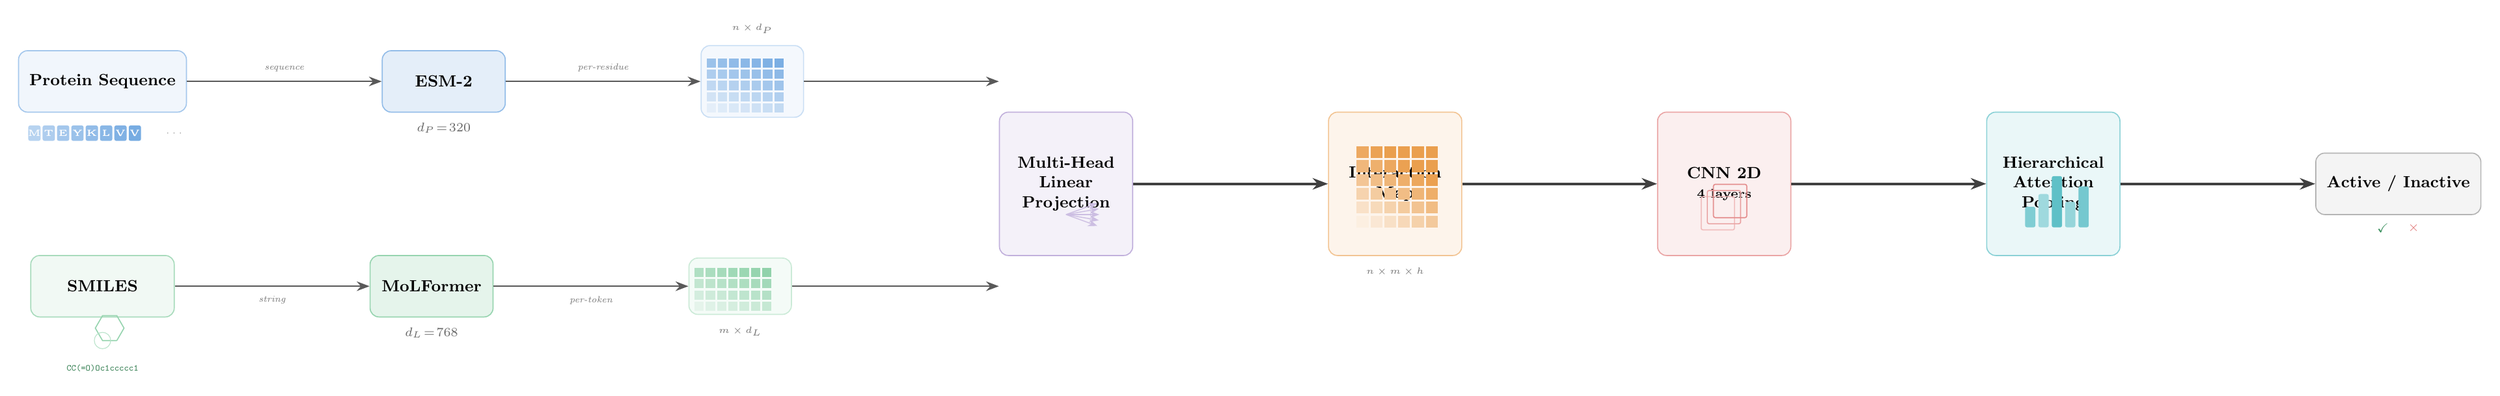
\begin{tikzpicture}[
  >=Stealth,
  % === ADJUSTABLE PARAMETERS ===
  % Modify these to fine-tune the layout:
  xsep/.store in=\xsep, xsep=3.8,       % horizontal gap between modules
  ysep/.store in=\ysep, ysep=2.0,        % vertical distance (protein↔ligand)
  boxw/.store in=\boxw, boxw=2.4,        % module box width
  boxh/.store in=\boxh, boxh=1.2,        % module box height (small)
  tallh/.store in=\tallh, tallh=2.8,     % module box height (tall, central)
  inpw/.store in=\inpw, inpw=2.8,        % input box width
  % === STYLES ===
  mod/.style={draw, rounded corners=5pt, minimum height=#1,
              minimum width=\boxw cm, font=\small\bfseries,
              inner sep=6pt, line width=0.6pt, align=center},
  mod/.default=\boxh cm,
  tall/.style={mod=\tallh cm, minimum width=2.6cm},
  inp/.style={mod, minimum width=\inpw cm},
  arr/.style={-{Stealth[length=2.5mm]}, line width=0.9pt, black!65},
  arrbold/.style={-{Stealth[length=3mm]}, line width=1.3pt, black!75},
  dim/.style={font=\tiny\itshape, text=black!55},
  lbl/.style={font=\scriptsize, text=black!60},
]

% === COLORS ===
\definecolor{protcol}{HTML}{4A90D9}
\definecolor{ligcol}{HTML}{50B87A}
\definecolor{projcol}{HTML}{8E6FBF}
\definecolor{mapcol}{HTML}{E8943A}
\definecolor{cnncol}{HTML}{D95B5B}
\definecolor{poolcol}{HTML}{2AABB5}
\definecolor{outcol}{HTML}{444444}

% =========================================================================
%  ROW 1: PROTEIN BRANCH (y = +ysep)
% =========================================================================

% (A) Protein Sequence input
\node[inp, fill=protcol!8, draw=protcol!50] (pseq) at (0, \ysep) {Protein Sequence};
% Amino acid strip — positioned relative to pseq
\foreach \i/\aa in {0/M, 1/T, 2/E, 3/Y, 4/K, 5/L, 6/V, 7/V} {
  \pgfmathsetmacro{\op}{40 + 5*\i}
  \fill[protcol!\op, rounded corners=1pt]
    ($(pseq.south west) + (0.2+\i*0.28, -0.55)$) rectangle ++(0.24, 0.30);
  \node[font=\tiny\bfseries, white]
    at ($(pseq.south west) + (0.32+\i*0.28, -0.40)$) {\aa};
}
\node[font=\tiny, text=black!40] at ($(pseq.south east) + (-0.25, -0.40)$) {$\cdots$};

% (B) ESM-2
\node[mod, fill=protcol!15, draw=protcol!60, right=\xsep cm of pseq] (esm) {ESM-2};
\node[lbl, below=2pt of esm] {$d_P\!=\!320$};

% (C) Protein embeddings
\node[mod, fill=protcol!6, draw=protcol!30, right=\xsep cm of esm,
      minimum width=2.0cm, minimum height=1.4cm] (pemb) {};
% Embedding matrix grid — relative to pemb
\foreach \i in {0,...,4} {
  \foreach \j in {0,...,6} {
    \pgfmathsetmacro{\op}{15 + 10*\i + 3*\j}
    \fill[protcol!\op]
      ($(pemb.south west) + (0.12+\j*0.22, 0.10+\i*0.22)$) rectangle ++(0.18, 0.18);
  }
}
\node[dim, above=3pt of pemb] {$n \times d_P$};

% =========================================================================
%  ROW 2: LIGAND BRANCH (y = -ysep)
% =========================================================================

% (D) SMILES input
\node[inp, fill=ligcol!8, draw=ligcol!50] (smi) at (0, -\ysep) {SMILES};
% Benzene ring — positioned relative to smi
\draw[ligcol!60, line width=0.6pt]
  ($(smi.south) + (0, -0.45)$) ++(0:0.28)
  \foreach \a in {60,120,...,360} {-- ++(\a:0.28)};
\draw[ligcol!40, line width=0.4pt] ($(smi.south) + (0, -0.45)$) circle (0.16);
\node[font=\tiny\ttfamily, text=ligcol!70!black, below=0.8cm of smi]
  {CC(=O)Oc1ccccc1};

% (E) MoLFormer
\node[mod, fill=ligcol!15, draw=ligcol!60, right=\xsep cm of smi] (mol) {MoLFormer};
\node[lbl, below=2pt of mol] {$d_L\!=\!768$};

% (F) Ligand embeddings
\node[mod, fill=ligcol!6, draw=ligcol!30, right=\xsep cm of mol,
      minimum width=2.0cm, minimum height=1.1cm] (lemb) {};
\foreach \i in {0,...,3} {
  \foreach \j in {0,...,6} {
    \pgfmathsetmacro{\op}{15 + 10*\i + 3*\j}
    \fill[ligcol!\op]
      ($(lemb.south west) + (0.12+\j*0.22, 0.08+\i*0.22)$) rectangle ++(0.18, 0.18);
  }
}
\node[dim, below=3pt of lemb] {$m \times d_L$};

% =========================================================================
%  CENTRAL PIPELINE (y = 0, right of embeddings)
% =========================================================================

% (G) Multi-Head Linear Projection
\node[tall, fill=projcol!10, draw=projcol!55,
      right=\xsep cm of pemb, yshift=-\ysep cm] (proj)
  {Multi-Head\\Linear\\Projection};
% Fan-out arrows inside — relative to proj
\foreach \a in {-20,-10,0,10,20} {
  \draw[projcol!45, line width=0.5pt, ->]
    ($(proj.center) + (0, -0.6)$) -- +(\a:0.65);
}

% (H) Interaction Map
\node[tall, fill=mapcol!10, draw=mapcol!55,
      right=\xsep cm of proj] (imap) {Interaction\\Map};
% Heatmap grid — relative to imap
\foreach \i in {0,...,5} {
  \foreach \j in {0,...,5} {
    \pgfmathsetmacro{\heat}{int(15 + 13*\i + 7*\j)}
    \pgfmathsetmacro{\heatclip}{min(\heat, 90)}
    \fill[mapcol!\heatclip]
      ($(imap.center) + (-0.75+\j*0.27, -0.85+\i*0.27)$) rectangle ++(0.23, 0.23);
  }
}
\node[dim, below=3pt of imap] {$n \times m \times h$};

% (I) CNN 2D
\node[tall, fill=cnncol!10, draw=cnncol!55,
      right=\xsep cm of imap] (cnn) {CNN 2D\\{\scriptsize 4 layers}};
% Stacked filter visual — relative to cnn
\foreach \dx/\dy/\op in {0/0/40, 0.12/0.12/55, 0.24/0.24/70} {
  \draw[cnncol!\op, line width=0.6pt, rounded corners=1pt]
    ($(cnn.center) + (-0.45+\dx, -0.9+\dy)$) rectangle ++(0.65, 0.65);
}

% (J) Hierarchical Attention Pooling
\node[tall, fill=poolcol!10, draw=poolcol!55,
      right=\xsep cm of cnn] (pool) {Hierarchical\\Attention\\Pooling};
% Bar chart visual — relative to pool
\foreach \i/\h/\op in {0/0.40/60, 1/0.65/45, 2/1.00/75, 3/0.50/50, 4/0.80/65} {
  \fill[poolcol!\op, rounded corners=1pt]
    ($(pool.center) + (-0.55+\i*0.26, -0.85)$) rectangle ++(0.20, \h);
}

% (K) Output
\node[mod, fill=outcol!6, draw=outcol!40, minimum width=2.4cm,
      right=\xsep cm of pool] (out) {Active / Inactive};
% Checkmark & X — relative to out
\node[font=\scriptsize, text=ligcol!80!black] at ($(out.south) + (-0.3, -0.25)$) {\checkmark};
\node[font=\scriptsize, text=cnncol!80] at ($(out.south) + (0.3, -0.25)$) {$\times$};

% =========================================================================
%  ARROWS
% =========================================================================
% Protein branch
\draw[arr] (pseq.east) -- (esm.west);
\draw[arr] (esm.east)  -- (pemb.west);
\draw[arr] (pemb.east)  -- (proj.west |- pemb.east);   % enter proj at protein height

% Ligand branch
\draw[arr] (smi.east) -- (mol.west);
\draw[arr] (mol.east)  -- (lemb.west);
\draw[arr] (lemb.east) -- (proj.west |- lemb.east);    % enter proj at ligand height

% Central pipeline (bold)
\draw[arrbold] (proj.east) -- (imap.west);
\draw[arrbold] (imap.east) -- (cnn.west);
\draw[arrbold] (cnn.east)  -- (pool.west);
\draw[arrbold] (pool.east) -- (out.west);

% =========================================================================
%  EDGE LABELS
% =========================================================================
\node[dim, above=2pt] at ($(pseq.east)!0.5!(esm.west)$) {sequence};
\node[dim, above=2pt] at ($(esm.east)!0.5!(pemb.west)$) {per-residue};
\node[dim, below=2pt] at ($(smi.east)!0.5!(mol.west)$)  {string};
\node[dim, below=2pt] at ($(mol.east)!0.5!(lemb.west)$)  {per-token};

\end{tikzpicture}
\end{document}
